\section{Implementierung}\label{sec:06_04_implementierung}
Die wesentliche Eigenschaft des bereitgestellten Kommunikationsmodells ist, dass es Beziehungen beinhaltet, welche jeweils durch einen Sender, einen Empfänger und eine Gewichtung repräsentiert werden. 
Die natürliche Struktur der Daten spiegelt ganz offensichtlich die eines gerichteten Graphen wieder. 
Die Speicherung der Daten in einer Graph-Datenbank ermöglicht die direkte Erkennung ihrer immanenten Beziehungen, was bei tabellenartigen (SQL) oder dokumentenbasierten (NoSQL) Datenbanken ohne komplexe Anfragen deutlich schwieriger ist. 
Die Applikation entspricht also einer ETL\footnote{Extract, Transform, Load}-Pipeline. Sie bezieht sich auf die Erfassung von Daten aus einem externen System und deren Überführung in einem domänespezifischen
Format, das das Abfragen und die Analyse der Daten erleichtert. 
\begin{figure}[H]
    \centering
    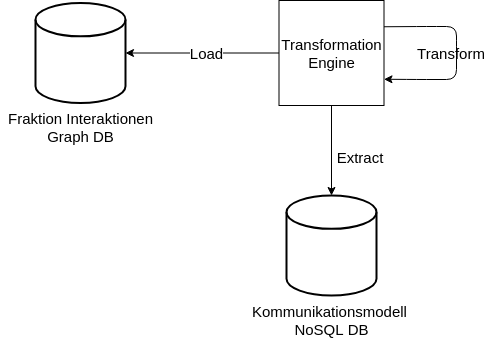
\includegraphics[width=0.60\textwidth]{images/ETL_Factions.png}
    \caption{Allgemeiner ETL-Prozess zur Erfassung, Transformation und zum Laden von Daten}
    \label{fig:faction-etl}
\end{figure}
In diesem Fall handelt es sich um die Erfassung von Dokumenten, also Sitzungen des Bundestags, und deren Transformierung in einen gerichteten Graphen, dessen Knoten und Kanten jeweils die 
Fraktionen der gesamten Legislaturperiode und ihre gegenseitige Interaktionen sind. Abbildung \ref{fig:faction-etl} stellt eine grobe Architektur der ETL-Pipeline dar.\\
Die Anwendung besteht aus vier Komponenten - eine Komponente pro Phase in der Pipeline und eine HTTP-Schnittstelle zum Auslösen des gesamten Vorgangs, wenn neue Daten vorhanden sind.
\begin{figure}[H]
    \centering
    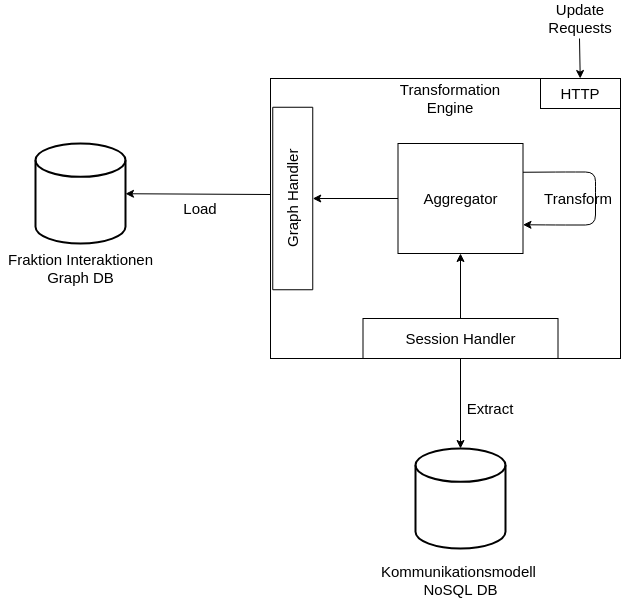
\includegraphics[width=0.60\textwidth]{images/ETL_Factions_Detail.png}
    \caption{ETL-Architektur der Applikation}
    \label{fig:faction-etl-app}
\end{figure}  
\subsection{Erfassung}
Die Kommunikation mit der externen Datenbank erfolgt über den sogenannten \textbf{Session Handler}, wie Abbildung \ref{fig:faction-etl-app} darstellt.
Er stellt zwei komplexe Anfragen an die Datenbank, damit die Sitzungen in einer passenden Form in das Programm eingeladen werden können.\\  
Die erste Anfrage gruppiert alle an einer Sitzung teilnehmende Abgeordneten nach der Fraktion der sie angehören.
Auf diese Weise wird eine Hash-Tabelle erstellt, deren Schlüssel und Werte jeweils die Bezeichner der Fraktionen und die Liste mit den zugehörigen Bezeichnern der Abgeordneten ist:
\begin{equation}
    \begin{aligned}
        \label{math:faction-hash-table}
        F_{1}^{(i)} &\rightarrow [A_{1}^{(1)}, A_{1}^{(2)}, \dots ,A_{1}^{(N_{1}^{(i)})}]\\
        F_{2}^{(i)} &\rightarrow [A_{2}^{(1)}, A_{2}^{(2)}, \dots ,A_{2}^{(N_{2}^{(i)})}]\\
            &\vdots\\
        F_{m}^{(i)} &\rightarrow [A_{m}^{(1)}, A_{m}^{(2)}, \dots ,A_{m}^{(N_{m}^{(i)})}].
    \end{aligned}
\end{equation}
$F_{m}^{(i)}$ ist die $m$-te Fraktion in der $i$-ten Sitzung und $A_{m}^{(1)}$ das erste Fraktionsmitglied der $m$-ten Fraktion.
$N_{m}^{(i)}$ ist der Anzahl aller Fraktionsmitglieder der $m$-ten Fraktion in der $i$-ten Sitzung.\\
Die zweite Anfrage aggregiert die Interaktionen, je nachdem ob eine Person oder eine Fraktion die Interaktion begonnen bzw. empfangen hat. 
Auf diese Weise können die unterschiedliche Arten von Beziehungen separat behandelt werden, was die Lesbarkeit des Quellcodes wesentlich erhöht.
Die Arten der Beziehungen wurden über Regular Expressions determiniert.\\
Das erfasste Datenmodell sah wie folgt aus: 
\begin{verbatim}
    class Faction:
        faction_id: str,
        name: str,
        members: list
        
    class Session:
        session_id: str, 
        legislative_period: int, 
        start_date: str,
        end_date: str, 
        pers_to_pers_comments: list, 
        fac_to_pers_comments: list, 
        pers_to_fac_comments: list,
        factions: List[Faction]
\end{verbatim}
\subsection{Transformierung}
Mittels \ref{math:faction-hash-table} kann eine Repräsentation für eine Fraktion in einer gesamten Legislaturperiode $L$ abgeleitet werden.
\begin{equation}
    \begin{aligned}
    \label{math:faction-size-union}
    F_{m}^{L} = \cup_{i=1}^{L} F_{m}^{(i)}.
    \end{aligned}
\end{equation}
\ref{math:faction-size-union} vereinigt sukzessiv die eindeutigen Fraktionsmitglieder der $m$-ten Fraktion aus jeder Sitzung. Das bedeutet, dass $N_m^{L}$ der Gesamtanzahl
aller Fraktionsmitglieder in Legislaturperiode $L$ entspricht. Somit sind alle Variablen zur Berechung der Gewichtungen vorhanden.\\
Der \textbf{Aggregator} (siehe Abbildung \ref{fig:faction-etl}) iteriert über jede Interaktion, berechnet die Gewichtung und führt alle Eigenschaften der
Interaktion zusammen mit der Gewichtung in einem Objekt über, das als eine Beziehung in einer Graph-Datenbank gespeichert werden kann. 
\subsection{Laden}
Die Anzahl der Kommentare in einer Legislaturperiode beträgt i.d.R mehrere Hunderttausend (c.a $300 000$ für die 19. Legislaturperiode). 
Die Speicherkapazität eines durchschnittlichen Rechners ist ungenügend, um alle Kommentare gleichzeitig in RAM aufzubewahren oder alle Kommentare auf einmal 
in der Graph-Datenbank zu speichern. Aus diesem Grund werden die Sitzungen hintereinander verarbeitet, wobei die Kommentare in einer Sitzung schubweise 
an die Graph-Datenbank weitergegeben werden.

\subsection{Abfrage}
Folgende Abfrage gibt eine Tabelle aus, die die aggregierten Sentiments zwischen allen Fraktionen angibt.
%\begin{minted}{cypher}
\begin{verbatim}
MATCH p=(sender:Faction)-[r:COMMENTED]->(receiver:Faction) 
WITH sender, receiver, sum(r.weight) AS weightsum,
	collect(r) AS rlist 
UNWIND rlist as r 
RETURN sender.name, receiver.name,
	sum((r.weight/weightsum)*r.polarity)
\end{verbatim}

%\end{minted}

Dazu werden zuerst alle Relationen mit einzigartigem Sender und Empfänger gruppiert und deren Gewichtssumme ausgerechnet. In diesem Schritt werden alle Relationen auch zu einer Liste zusammengefasst. Das ist notwendig, da in einer WITH expression alle Ausgaben die gleiche Anzahl an Werten für einen Grouping Key zurückgeben müssen. In diesem Fall wird jedem Sender-Empfängerpaar eine Gewichtssumme und eine Relationsliste zugeordnet, welche dann weiterverarbeitet wird. Im nächsten Schritt wird die Relationsliste wieder in ihre Elemente zerlegt um die sum() Akkumulationsfunktion benutzen zu können. Das Resultat der Query ist dann der gewichtete Sentimentmittelwert für jedes Sender-Empfänger-Paar.


%implementierung der berechnung der gesamtsentiments als query
